\section{Notes}

Static variables

Global variables

Volatile

extern


\textbf{Build process}



\subsection{Interrupts}
An interrupt is the automatic transfer of software execution in response to a hardware event that is asynchronous with the current software execution.

The hardware event is called a trigger. When this happens, an ISR is called.
This pauses the execution of the regular code, until the ISR returns or a
higher priority interrupt is triggered.


\subsection{Task model}
A task is an independent thread of execution that can compete with
other concurrent tasks for processor execution time.
It is the same as a process in a multitasking operating system.

\textbf{Division of applications into tasks}

Criteria for task creation:

\begin{itemize}
	\item{Parallelism: Simultaneous and independent functionality}
	\item{Timing: Different timing constraints}
	\item{Priority: Divide tasks with different priority}
	\item{Structure: Each task handles one well defined problem}
	\item{Coupling: Divide problem into loosely coupled tasks.}
	\item{Periodicity: A task that must execute with a fixed period is a task by itself.}
\end{itemize}

\begin{center}
	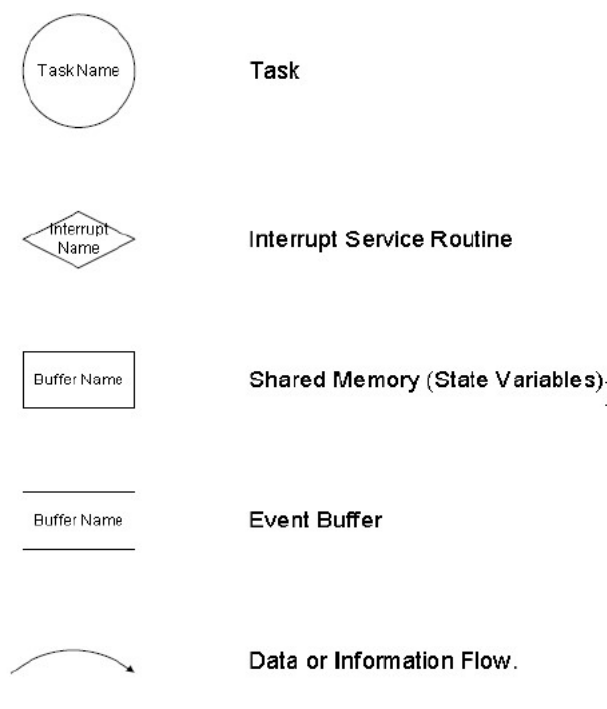
\includegraphics[width=0.4\textwidth]{images/taskDiagramComponents.png}
\end{center}

A shared memory element keeps its value after it has been read.
An event from the event buffer gets destroyed after reading and processing.

